\chapter{Teakwood System }

\section{Overview}
Structurally, like most websites, Teakwood system has a three layers layout: frontend, backend, and database. Becuase Teakwood will use computing servers to run jobs, so the eco Teakwood system actually has four layers, the up mentioned three plus the computing layer. the below figure shows how it looks like:\\

\begin{figure}[htb]
\centering
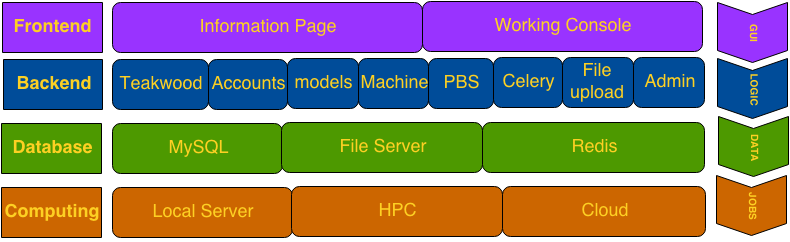
\includegraphics[scale=0.5]{./system_structure} 
% e.g. insert ./image for image.png in the working directory, adjust scale as necessary
\caption{Teakwood System Overview}
\label{fig:label} % insert suitable label, this is used to refer to a fig from within the text as shown above
\end{figure}

On the above figure, we can see four straight layers bottom up. In each layer, the left part is the layer name, the middle part is the layer content, and the right part is layer reality. Let's go through these layers one by one.

\section{Frontend}
The frontend is a visible GUI that user interact with. Basically all what we can see from the Teakwood website can be called "frontend".  For neat purpose, Teakwood separated the frontend into two parts: the \textbf{information page} and the \textbf{working console}. See below:

\begin{figure}[htb]
\centering
%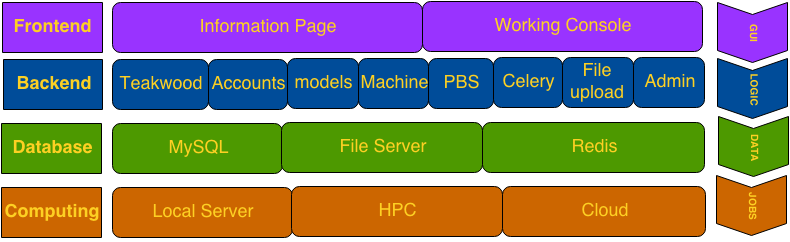
\includegraphics[scale=0.5]{./system_structure} 
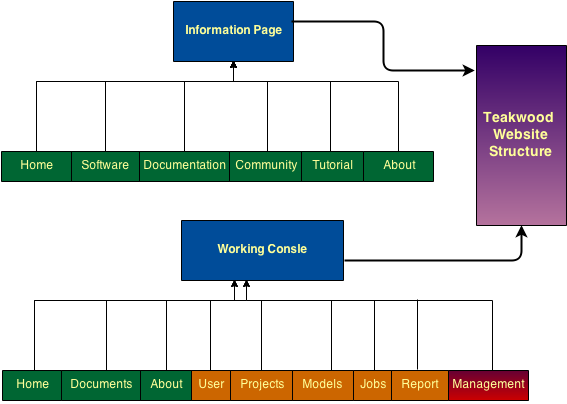
\includegraphics[scale=0.6]{./website_structure} % e.g. insert ./image for image.png in the working directory, adjust scale as necessary
\caption{Website Strucutre}
\label{fig:label} % insert suitable label, this is used to refer to a fig from within the text as shown above
\end{figure}

The \textbf{information page} introduces you all things about Teakwood.\\

$\bullet$ What is teakwood?\\
$\bullet$ What can Teakwood do?\\
$\bullet$ How to install Teakwood?\\
$\bullet$ How to use Teakwood?\\
$\bullet$ The user manual.\\
$\bullet$ Video tutorial.\\
$\bullet$ Teakwood forum.\\


The \textbf{working console} is your working place where you tango with your jobs and data. The functions buttons guide you to different places.\\

$\bullet$ \textbf{User}: Display user information.\\
$\bullet$ \textbf{Projects}: Create project and overview project.\\
$\bullet$ \textbf{Models}: Create model and overview model.\\
$\bullet$ \textbf{Jobs}:Create jobs, overview jobs and job monitoring.\\
$\bullet$ \textbf{Report}:Download job output.\\
$\bullet$ \textbf{Management}:Access to the admin system.\\


Note the color differences in the bottom layer.\\

$\bullet$ The \textbf{Green}: all visitors can see and manipulate.\\
$\bullet$ The \textbf{orange}: only logging user can see and manipulate.\\
$\bullet$ The \textbf{red}: only superuser can see and manipulate.\\


\section{Backend}
The backend is the logical design on how to interact with user. This Includes verifying user's request, pulling requested data, generating HTML web page and displaying web page. Teakwood follows the MVC(Model-View-Controller)design pattern and separates all the functions in to loose coupling parts, in Django, it call "app". All parts can both work independently and cooperatively.(We will have a backend chapter to reveal the logic mystery.)

In Teakwood system, there are mainly eight parts(Apps).\\

$\bullet$ \textbf{Teakwood}: control the frontend presentation.\\
$\bullet$ \textbf{Accounts}: control the user identification.\\
$\bullet$ \textbf{Models}: invoke and control the computing models.\\
$\bullet$ \textbf{machine}:invoke and control the computing resources\\
$\bullet$ \textbf{PBS}:Guide the PBS script generation.\\
$\bullet$ \textbf{File upload}:gather input files to buffer for downloading \\
$\bullet$ \textbf{Admin}:overall control of user and data.\\
$\bullet$ \textbf{Celery}:asynchronous handling.\\

\section{Data handling}
Teakwood system handles three types of data: the website data, the computing data and the message queue data. For each type of data we provide a different storage. see this table:\\
\\   
\begin{table}[h]
\begin{tabular}{lllll}
\cline{1-3}
\multicolumn{1}{|c|}{\textbf{Website data}} & \multicolumn{1}{c|}{\textbf{Computing data}} & \multicolumn{1}{c|}{\textbf{Message queue data}} &  &  \\ \cline{1-3}
\multicolumn{1}{|c|}{\textbf{MySQL}} & \multicolumn{1}{c|}{\textbf{File server}} & \multicolumn{1}{c|}{\textbf{redis server}} &  &  \\ \cline{1-3}
\multicolumn{1}{|c|}{\textbf{Teakwood data}} & \multicolumn{1}{c|}{\textbf{inputs and outputs}} & \multicolumn{1}{c|}{\textbf{Asynchronous handling}} &  &  \\ \cline{1-3}
                                &                                &                                &  & 
\end{tabular}
\end{table}


Teakwood website uses MySQL database for store it website data, e.g. the user account and the project labels.\\
For the computing data, we periodically rsync them to a separate file server for data  backup and downloading purpose. e.g. input files and the output result.\\
Message queue data is generated when we use Celery to asynchronous processing time consuming process. They are just ephemeral data, so we simply use a redis server to keep it.\\

\section{Remote Configuration}
Before the first time we can run a job in HPC or cloud, we have set up a connection and ready everything. the main things we should done are:\\

$\bullet$ Establish an password-less ssh log-in.\\
$\bullet$ Compile the tools and packages we will use in remote machine.\\
$\bullet$ Ready all the import path for Teakwood to use.\\

One those steps are done, we just simply "plug-in" Teakwood to the remote machine, and everything we can do from Teakwood web portal, without touch the under layers.


%\subsection{<Sub-section title>}

%\subsection{<Sub-section title>}
%some text\cite{citation-2-name-here}, some more text

%Refer figure \ref{fig:label}.


